\section{Supplement}
%===================================================================================================
\subsection{Data \& Code}\label{app.data}
Table~\ref{tab:data} gives the RDS-adjusted data from \cite{Baral2014}.
All analysis code is available online at:\\
\hreftt{github.com/mishra-lab/duration-bias}
\begin{table}[h]
  \centering
  \caption{RDS-adjusted proportions for variables}
  \begin{tabular}{llrc}
  \toprule
  Variable           & Stratum & Mean & (\ci) \\
  \midrule
  Years selling sex
    & 0--2    & 38.3 & (27.5,~49.1) \\
    & 3--5    & 32.1 & (23.6,~40.7) \\
    & 6--10   & 20.2 & (13.2,~27.1) \\
    & 11+     &  9.4 & (04.4,~14.4) \\[1ex]
  New clients\tn{a}
    & 0--1    & 16.4 & (09.8,~23.0) \\
    & 2       & 43.4 & (33.3,~53.5) \\
    & 3       & 15.2 & (09.6,~20.9) \\
    & 4       & 13.1 & (07.0,~19.2) \\
    & 5       & 11.8 & (06.0,~17.6) \\[1ex]
  Regular clients\tn{a}
    & 0--1    & 10.0 & (01.9,~18.1) \\
    & 2       &  8.5 & (03.2,~13.8) \\
    & 3       & 15.9 & (09.8,~21.9) \\
    & 4       & 10.0 & (04.5,~15.6) \\
    & 5       &  8.1 & (03.8,~12.3) \\
    & 6       & 10.7 & (05.8,~15.5) \\
    & 7+      & 36.9 & (26.4,~47.3) \\[1ex]
  Non-paying partners\tn{a} 
    & 0       & 12.5 & (04.8,~20.1) \\
    & 1       & 50.8 & (42.9,~58.7) \\
    & 2       & 23.6 & (16.8,~30.3) \\
    & 3+      & 13.2 & (07.2,~19.1) \\
  \bottomrule
\end{tabular}
\floatfoot{\vskip1ex\centering%
  \tnt[a]{Number reported in the past 30 days.}
  Data from \cite{Baral2014}.}

  \label{tab:data}
  \floatfoot{
    \tnt[a]{Number reported in the past 30 days.}
    Data from \cite{Baral2014}.}
\end{table}
%===================================================================================================
\subsection{Beta Approximation of the Binomial Distribution}\label{app.bab}
The distributions of RDS-adjusted variables in \cite{Baral2014} were reported as
adjusted proportions (mean, \ci) for different variable value strata.
For each proportion, we defined a beta approximation of the binomial (BAB) distribution:
\begin{alignat}{1}\label{eq:bab}
  \distr{P}{\rho} &=
    \frac{\Gamma(\alpha+\beta)}{\Gamma(\alpha)\,\Gamma(\beta)}\,
    \rho^{\alpha-1}{(1 - \rho)}^{\beta-1} \\
    &\approx {N \choose n} \, \rho^{n}{(1 - \rho)}^{N - n} \nonumber
\end{alignat}
with $\alpha = N\,\rho$ and $\beta = N\,(1-\rho)$.
We fixed $\rho$ as the adjusted point estimate,
and estimated $N$ by minimizing the sum of squared differences between
the 95\% quantiles of \eqref{eq:bab} given $N$ and the reported \ci for the adjusted proportion.
%===================================================================================================
\subsection{Risk Group Duration}\label{app.yss}
%---------------------------------------------------------------------------------------------------
\paragraph{Fitting to RDS-Adjusted Proportions}
\begin{figure}[h]
  \centering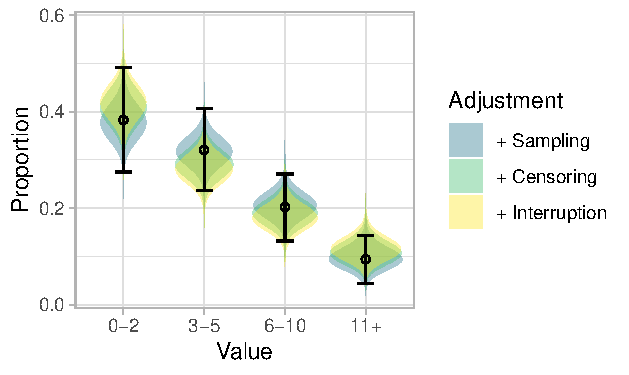
\includegraphics[scale=.8]{yss.fit}
  \caption{TODO}
  \floatfoot{TODO}
\end{figure}
%---------------------------------------------------------------------------------------------------
\paragraph{Numeric Summary}
Table~\ref{tab:yss.adj} summarizes the estimated exponential distribution means (\ci)
for years selling sex following each stage of adjustment outlined in \sref{meth.yss}.
\begin{table}[h]
  \centering
  \caption{Estimated mean durations selling sex (years) following each stage of adjustment}
  \begin{tabular}{lrc}
  \toprule
  Adjustment     & Mean & (\ci) \\
  \midrule
  Median         & 4.00 & --- \\
  Mean           & 5.77 & --- \\
  + Sampling     & 4.35 & (3.27,~\w5.72) \\
  + Censoring    & 9.40 & (6.60,~13.22) \\
  + Interruption & 4.06 & (2.29,~\w6.34) \\
  \bottomrule
\end{tabular}

  \label{tab:yss.adj}
\end{table}
%===================================================================================================
\subsection{Rate of Partnership Change}\label{app.partners}
%---------------------------------------------------------------------------------------------------
\paragraph{Fitting to RDS-Adjusted Proportions}
\begin{figure}[h]
  \centering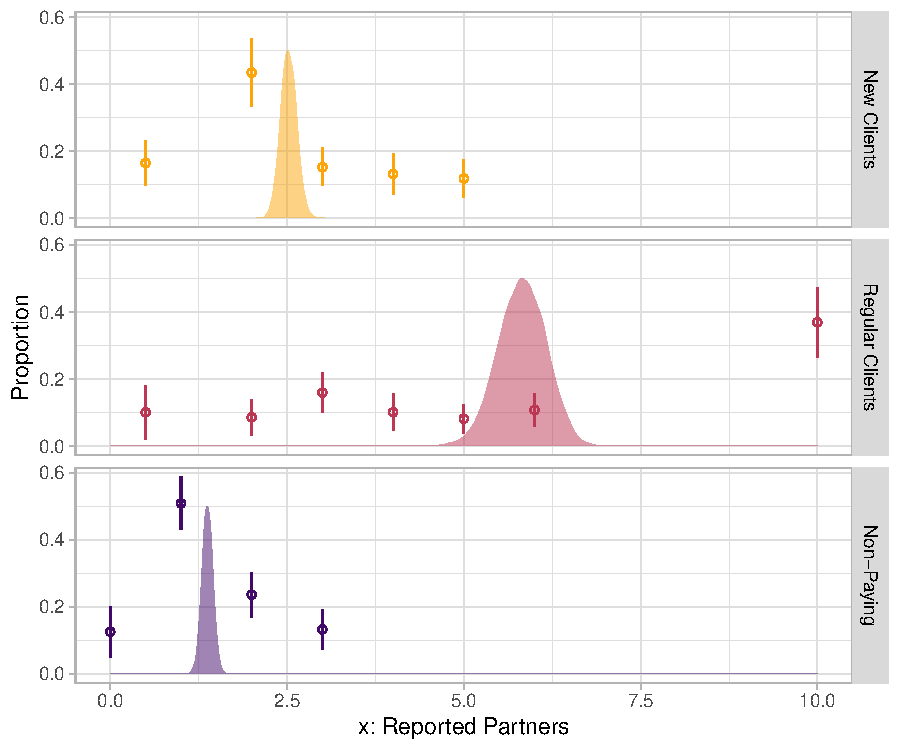
\includegraphics[scale=.8]{partners.fit}
  \caption{TODO}
  \floatfoot{TODO}
\end{figure}
%---------------------------------------------------------------------------------------------------
\paragraph{Numeric Summary}
\begin{table}[h]
  \centering
  \caption{Biased \vs unbiased estimates of
    rates of partnership change and numbers of current partners
    for three partnership types reported by female sex workers}
  \begin{tabular}{llrcrc}
  \toprule
   & & \multicolumn{2}{c}{Rate $Q$} &
       \multicolumn{2}{c}{Number $K$} \\
  \cmidrule(rl){3-4}\cmidrule(rl){5-6}
  Partnership Type & Bias & Mean & 95\%~CI & Mean & 95\%~CI \\
  \midrule
  New Clients     & Biased   & 1.77 & (1.65,\,1.89) & 1.77 & (1.65,\,1.89) \\
                  & Unbiased & 1.71 & (1.60,\,1.83) & 0.06 & (0.05,\,0.06) \\
  Regular Clients & Biased   & 4.69 & (4.49,\,4.89) & 4.69 & (4.49,\,4.89) \\
                  & Unbiased & 0.94 & (0.90,\,0.98) & 3.75 & (3.60,\,3.91) \\
  Non-Paying      & Biased   & 0.74 & (0.66,\,0.82) & 0.74 & (0.66,\,0.82) \\
                  & Unbiased & 0.02 & (0.02,\,0.02) & 0.72 & (0.64,\,0.80) \\
  \bottomrule
\end{tabular}

  \label{tab:partners.fsw}
  \floatfoot{Rares are per-month.}
\end{table}
